%=============================================================
% Header, Cover, and Preamble
%=============================================================
\documentclass[a4paper,english]{book}
%=============================================================
\usepackage{amsmath} %use package here for formulas, maybe needed
\usepackage{graphicx} % This for Images
\usepackage{babel}
\usepackage{makeidx}
\usepackage{index}
\usepackage{datetime}
%=============================================================
\makeindex
%=============================================================
\title{\textbf{Software Engineering Project Report}}
%-------------------------------------------------------------
\newdateformat{monthdayyeardate}{
	\monthname[\THEMONTH]~\THEDAY, \THEYEAR}
%=============================================================
% Begining of The Document
%=============================================================
\begin{document}
\author{Belal Hmedan \& Deng Jianning\\University Bourgogne}
%=============================================================
\maketitle
%=============================================================
\let\cleardoublepage\clearpage
%=============================================================
\tableofcontents
%=============================================================
% The Core of Report
%=============================================================
\chapter*{Introduction}
\addcontentsline{toc}{chapter}{Introduction} \markboth{INTRODUCTION}{}
This is an Introduction
%=============================================================
\chapter{Project Description}
\section{Goal of the Project}
\section{Completeness of the Project (Supported Features)}
\section{Dependencies and References}
Apart from STL, I’m using Boost Graph Library (BGL), which in turn depends on other Boost Library: Property Map, which in turn depends on other Boost Libraries, so I included the whole Boost Libraries at once.
\section{Data Sets Introduction}
%=============================================================
\chapter{Code Design and Structure}
%=============================================================
\section{Algorithm and Shortest Path Design}
This part of code organized in 3 different Classes, each of them contains Header, and Source File:
%-------------------------------------------------------------
\subsection{ MyGraphBuilder Class:}
This Class mainly handles data provided from our Data Structure represented by the Model which depends on the OSM file in its compressed format PBF.
This Class mainly takes the nodes included inside ways only from the
Model as an input, then builds Vertices and Edges Between Vertices to construct the Graph, which in turn will be as an input to the Next stage which is Dijkstra Algorithm.
The Graph in my approach is Adjacency List proposed by Boost Graph Library.
The need for this procedure comes from the fact that: finding shortest path will be implemented through an algorithm, and the algorithm deals with graph, so I wrote this class to build the desired Graph from the Data Structure we imported from OSM file.
The input for this Class is the Model (Data Structure) extracted from OSM file, 
And the Output is a Bidirectional weighted Graph.
Bidirectional, because it’s easy to implement, in case we want improve it to Directional Graph, we must do a complicated constrains, and check each Tag, to see the type of Transportation, and if the way was one direction, or bidirectional.
Weighted Graph: because we are calculating Euclidean Distance between the Nodes depending on Longitude, and Latitude.
%-------------------------------------------------------------
\subsection{ MyAlgorithm Class:}
This Class takes the Graph produced on the past class MyGraphBuilder, and the Source Node which we will start from, and runs Dijkstra Algorithm proposed by Boost Graph Library to Find the Shortest Path Between the Source Node, and all other Nodes in The Graph.
Special Function in this class called: getShortPath takes the destination Node, then returns the shortest path between the source and destination only.
In case that there was no path between nodes, the path (Vector) will contain only one default node, so we don’t face issues due to empty vector.
%-------------------------------------------------------------
\subsection{ ShortPath Class:}
This Class is just to reduce amount of code in the main window, it doesn’t do much, it just takes Source Node, Destination Node, and Model, then it builds the Graph From the Model using MyGraphBuilder Class, and Runs MyAlgorithm Class, and its special Function getShortPath, finally the output is our shortest path.

%=============================================================
\section{Data Manipulation}
\section{Rendering}
%============================================================
\section{Routing}
Routing on this approach is just on foot, it’s possible to add more transport methods later using Tag filtering, building different transport maps, Vertices, and Edges, but unfortunately time was short for this project ! .
Isolated Nodes which doesn’t belong to any way are not included in building the Graph, because our purpose is to find a way between two nodes, so I didn’t build the graph with all nodes, only connected nodes which belong to way.
Euclidean Distance between the Nodes is our way to assign weight to Edges between Nodes, and of course the Way or Path is nothing except group of sequential Edges between connected Nodes.
%============================================================
\section{GUI}
Running the Program that will show a window with a Menu and four buttons Source, Destination, Navigate, and Cancel.
%------------------------------------------------------------
\begin{center}
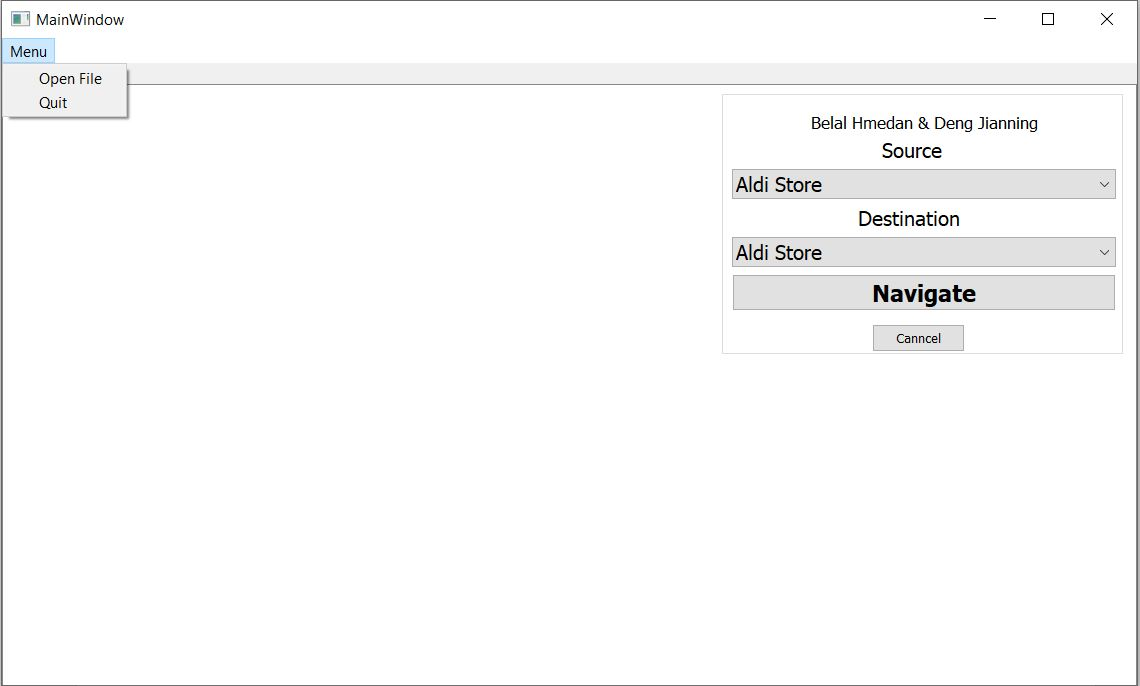
\includegraphics[width=.6\textwidth]{GUI_NoMap.JPG}
%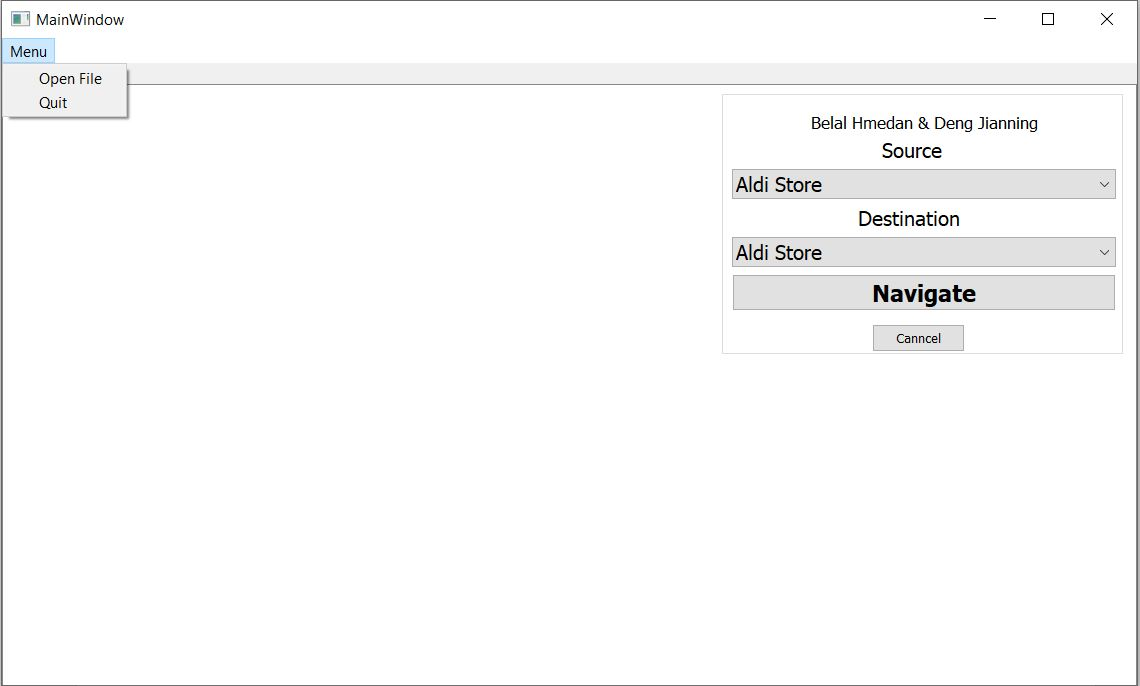
\includegraphics[width=.6\textwidth,natwidth=1200,natheight=700]{GUI_NoMap.JPG}
\end{center}
%------------------------------------------------------------
To start working, you should select (Menu - Open )
to open the map file, which should be with (.pbf) extension.
After you select your Map, the Software loads the map File showing the Map.
%------------------------------------------------------------
\begin{center}
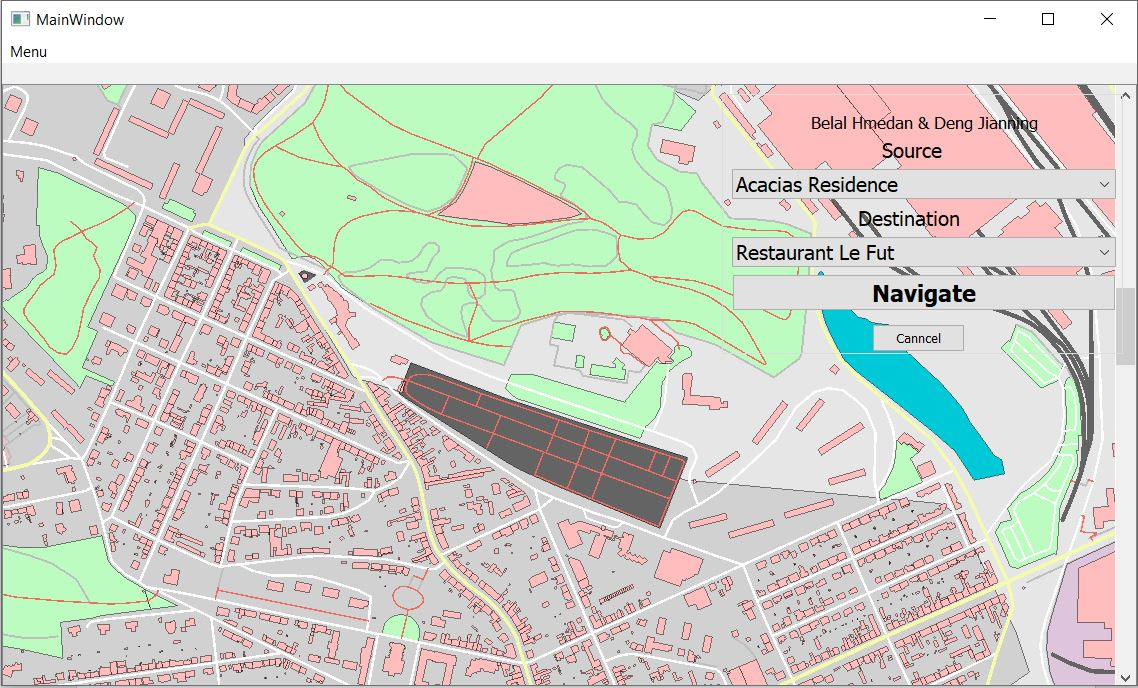
\includegraphics[width=.6\textwidth]{GUI_Map0.JPG}
%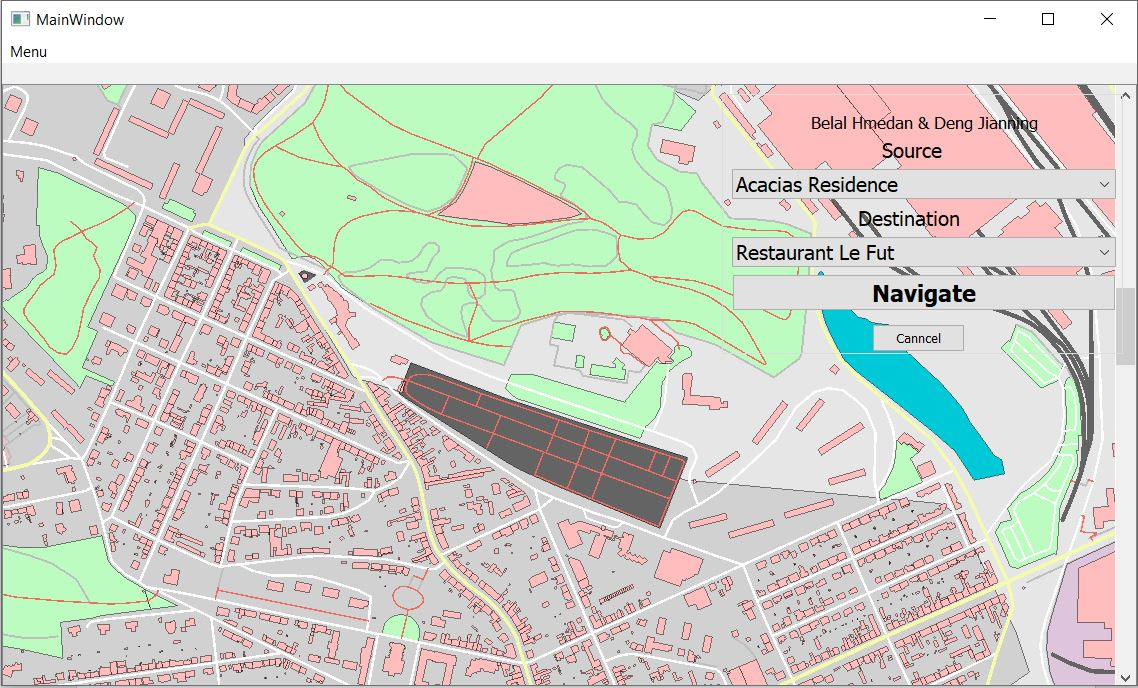
\includegraphics[width=.6\textwidth,natwidth=1200,natheight=700]{GUI_Map0.JPG}
\end{center}
%------------------------------------------------------------
The Dropdown lists Source, and Destination contains 20 places for each of them, All on Le Creusot City, where you can select your start point, and destination.
%------------------------------------------------------------
\begin{center}
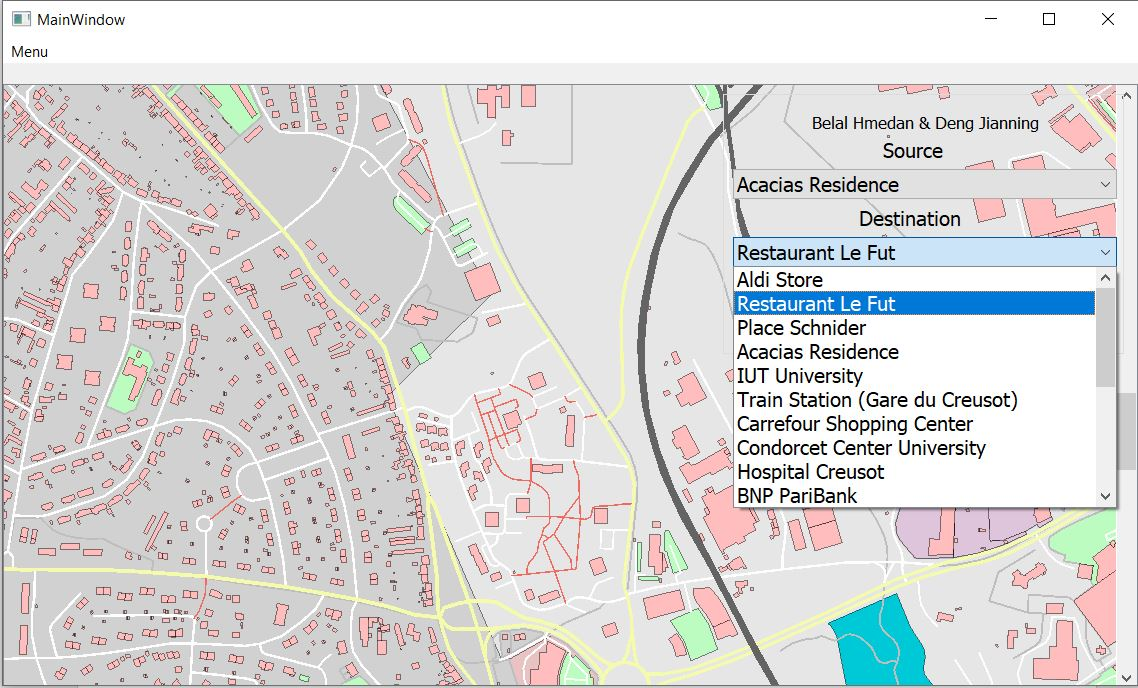
\includegraphics[width=.6\textwidth]{GUI_Map1.JPG}
%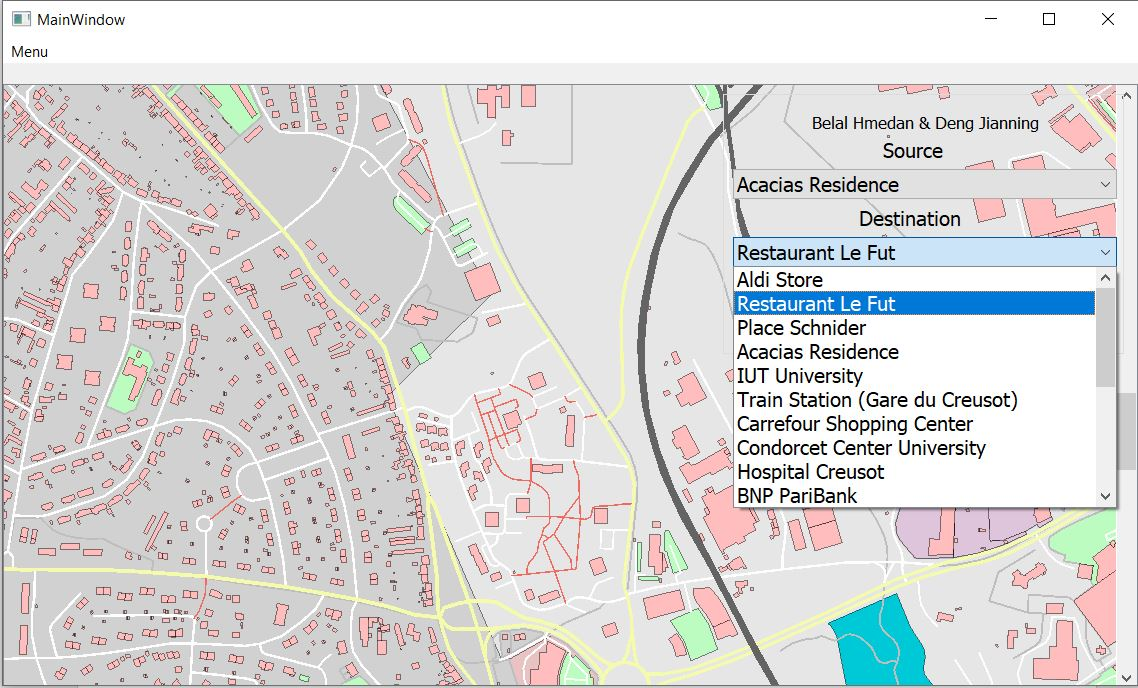
\includegraphics[width=.6\textwidth,natwidth=1200,natheight=700]{GUI_Map1.JPG}
\end{center}
%------------------------------------------------------------
by clicking on Navigate Button, the Shortest Path will be drawn by Red , so you can see the way you should follow.
%------------------------------------------------------------
\begin{center}
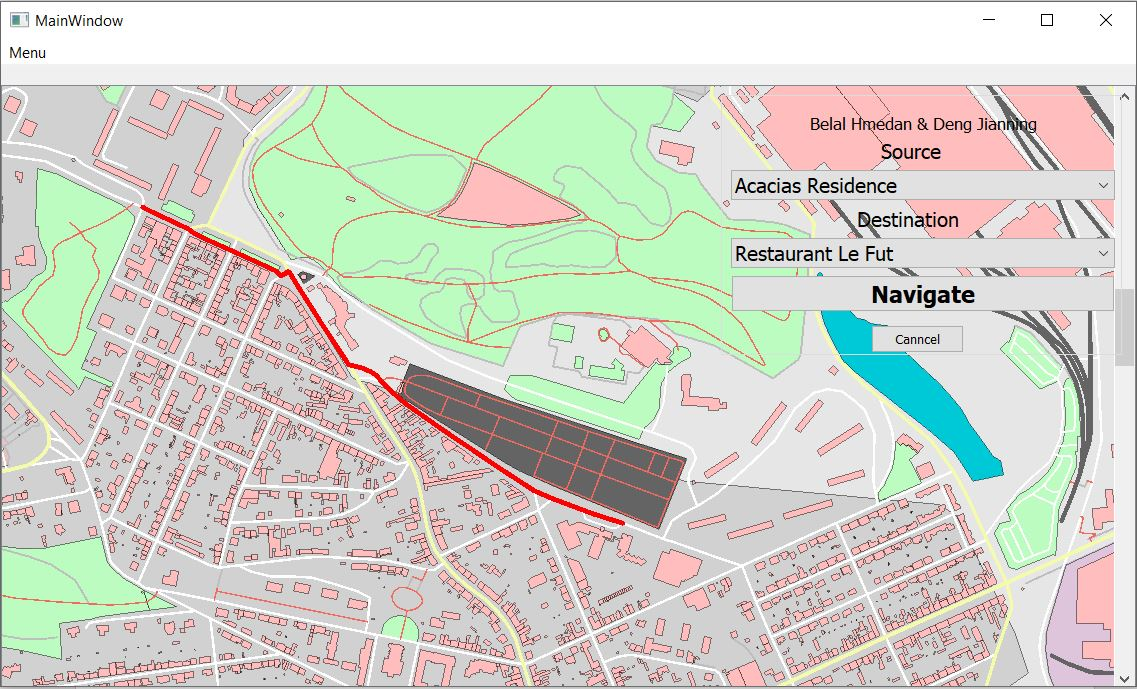
\includegraphics[width=.6\textwidth]{GUI_Map2.JPG}
%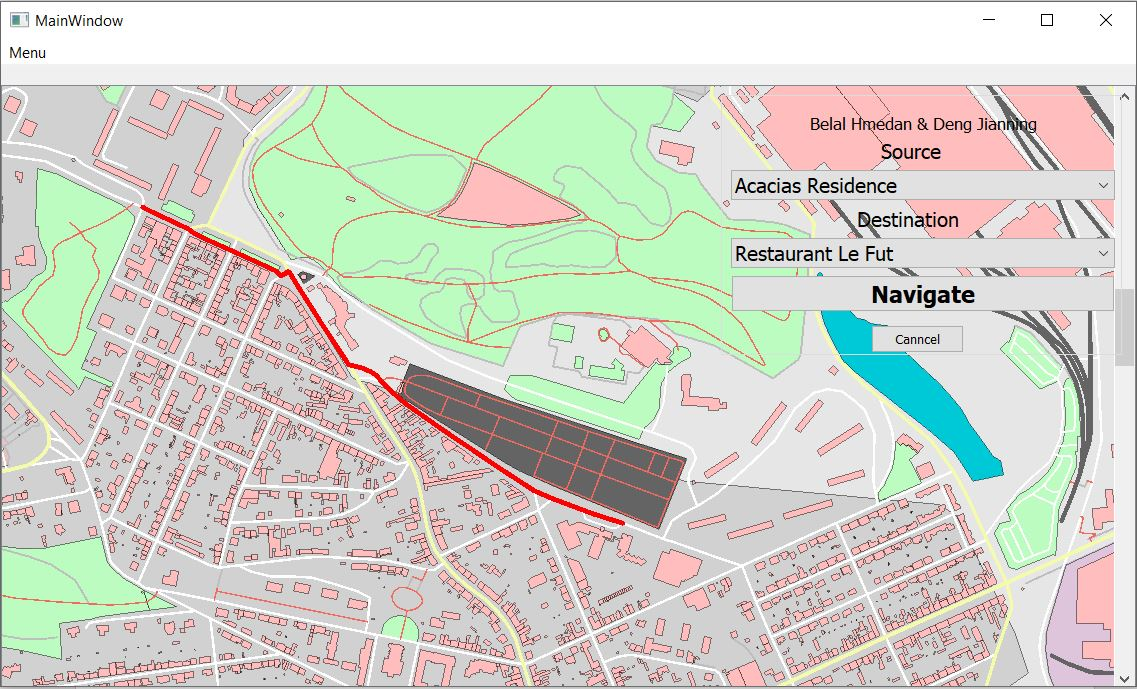
\includegraphics[width=.6\textwidth,natwidth=1200,natheight=700]{GUI_Map2.JPG}
\end{center}
%------------------------------------------------------------
Cancel button is to hide that path, and you can choose again your start point and target, so your path again will be drawn for you.
To Finish, you can select (Menu - Quit) to exit the Software.
%=============================================================
\section{problems during implementation:}
%=============================================================
There is two kind of Difficulties here:
\subsection{Problems we got rid of it:} 
\subsubsection{First Difficulty was CMake didn’t find some libraries:}
specially Boost Library, later we excluded Cmake, we depended on Headers only to implement our plan.
\subsubsection{Second Difficulty was that Edges can’t be built using idType Nodes:} the solution for that was mapping the idType Nodes to unsigned int indexes through a map, so each node has ID, and Vertex Number.
\subsubsection{Third one is Redundancy of Nodes in different Ways:} the solution was to compare each node of way to the map we built as solution to problem1.2, so if the node already found, we don’t add it to our map, instead we just call it and get Node index.

\subsection{Difficulties we can solve, but it needs more time:}
\subsubsection{1.Supporting Different Travel Method.}
\subsubsection{2.Building Directional Graph instead of Bidirectional one.}
\subsubsection{3.Adding Reviews, and stars options to the GUI.}
\subsubsection{4.Adding locations on the Map.}
%=============================================================
\chapter{Project Management}
\section{Overview of the Project Planning}
\section{Work Schedules}
\subsection{Plans VS Actual}
\section{Conclusion}
%=============================================================
\chapter{Summary}
%=============================================================
\begin{thebibliography}{12}
\bibitem{BGL} 
Jeremy G. Siek,
Lie-Quan Lee, Andrew Lumsdaine.
\textit{The Boost graph library : user guide and reference manual.} , ``Book," \emph{BGL}, pp. 161-322,Pearson Education, Inc., Reading, Massachusetts, 2002.
\end{thebibliography}
%=============================================================
\end{document}